\documentclass[border=2pt]{standalone}
\usepackage[T1]{fontenc}
\usepackage{lmodern}
\usepackage{amsmath}
\usepackage[siunitx]{circuitikz}
\usetikzlibrary{patterns,arrows.meta,calc,decorations.pathmorphing}
\definecolor{cBlue}{HTML}{2A78D6}
\definecolor{cOrange}{HTML}{EB6834}
\definecolor{cYellow}{HTML}{EDA100}
\definecolor{cAqua}{HTML}{1BAF7A}
\definecolor{cTxt}{HTML}{0B0B0B}
\definecolor{cTxt2}{HTML}{52514E}
\definecolor{cGrid}{HTML}{E6E5E1}
\ctikzset{bipoles/length=0.95cm}
\tikzset{
  dim/.style={{Latex[length=1.6mm]}-{Latex[length=1.6mm]},thin,cTxt2},
  lab/.style={font=\footnotesize,text=cTxt},
  lab2/.style={font=\footnotesize,text=cTxt2},
  ground/.style={pattern=north east lines,pattern color=cTxt2,draw=none},
}
% beam shape: y(s) = Y (3 s^2 - s^3)/2, s in [0,1], x = x0 + Lb s
\def\xz{0.3}\def\Lb{6.2}\def\Ytip{0.9}
\begin{document}
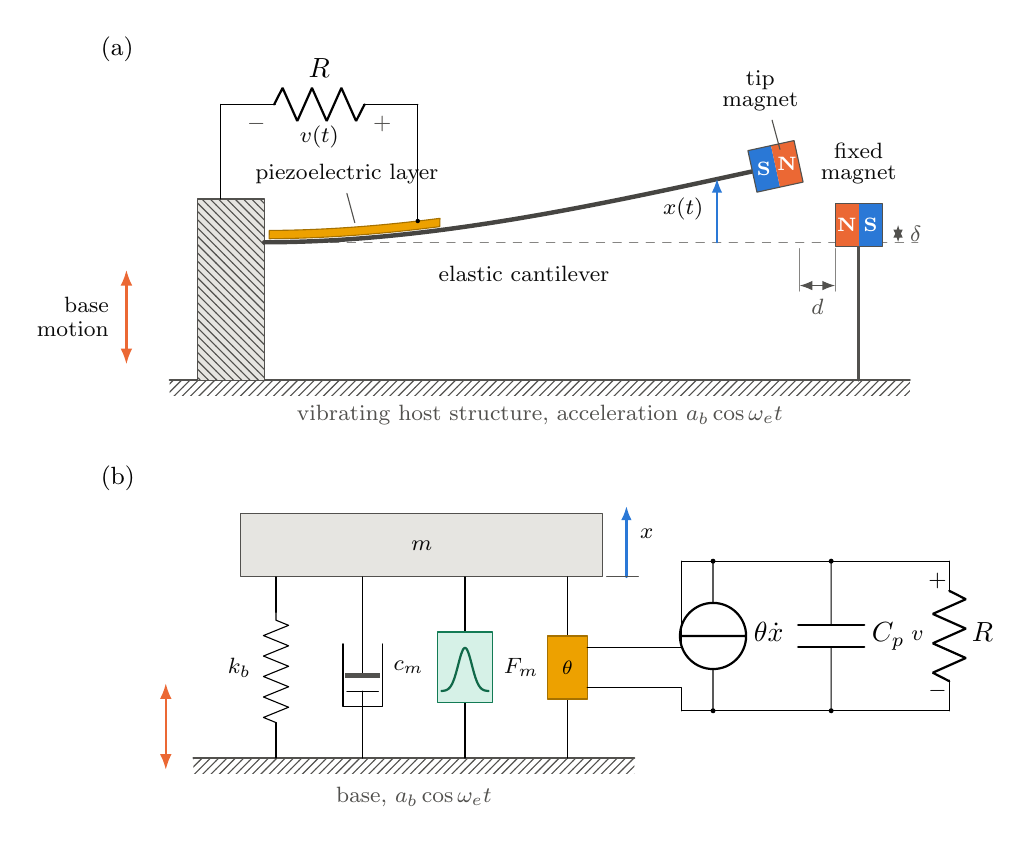
\begin{tikzpicture}[line cap=round,line join=round]
%% ============ panel (a): device ============
\node[font=\small,anchor=west] at (-1.9,2.45) {(a)};
% moving base
\fill[ground] (-0.9,-1.95) rectangle (8.5,-1.75);
\draw[thick,cTxt2] (-0.9,-1.75) -- (8.5,-1.75);
\draw[{Latex[length=2mm]}-{Latex[length=2mm]},thick,cOrange] (-1.45,-1.55) -- (-1.45,-0.35);
\node[lab,anchor=east,align=right] at (-1.55,-0.95) {base\\[-1pt] motion};
\node[lab2,anchor=north] at (3.8,-1.95) {vibrating host structure, acceleration $a_b\cos\omega_e t$};
% clamp
\fill[cGrid,draw=cTxt2] (-0.55,-1.75) rectangle (\xz,0.55);
\fill[pattern=north west lines,pattern color=cTxt2] (-0.55,-1.75) rectangle (\xz,0.55);
% undeformed axis
\draw[dashed,cTxt2!70,thin] (\xz,0) -- (8.6,0);
% piezoelectric layer on top of the root region (follows the beam)
\fill[cYellow,draw=cYellow!70!black,thin]
  plot[domain=0.01:0.36,samples=30] ({\xz+\Lb*\x},{\Ytip*(3*\x*\x-\x*\x*\x)/2+0.045})
  -- plot[domain=0.36:0.01,samples=30] ({\xz+\Lb*\x},{\Ytip*(3*\x*\x-\x*\x*\x)/2+0.15}) -- cycle;
% beam
\draw[line width=1.6pt,cTxt2!85!black] plot[domain=0:1,samples=60] ({\xz+\Lb*\x},{\Ytip*(3*\x*\x-\x*\x*\x)/2});
% tip magnet (rotated with the tip slope)
\begin{scope}[shift={(\xz+\Lb,\Ytip)},rotate=12.3]
  \fill[cBlue] (0,-0.27) rectangle (0.3,0.27);
  \fill[cOrange] (0.3,-0.27) rectangle (0.6,0.27);
  \draw[cTxt2,thin] (0,-0.27) rectangle (0.6,0.27);
  \node[font=\scriptsize\bfseries,white] at (0.15,0) {S};
  \node[font=\scriptsize\bfseries,white] at (0.45,0) {N};
\end{scope}
% fixed magnet, offset delta, like poles facing
\def\yd{0.22}
\draw[line width=1.2pt,cTxt2] (7.85,\yd-0.27) -- (7.85,-1.75);
\fill[cOrange] (7.55,\yd-0.27) rectangle (7.85,\yd+0.27);
\fill[cBlue] (7.85,\yd-0.27) rectangle (8.15,\yd+0.27);
\draw[cTxt2,thin] (7.55,\yd-0.27) rectangle (8.15,\yd+0.27);
\node[font=\scriptsize\bfseries,white] at (7.70,\yd) {N};
\node[font=\scriptsize\bfseries,white] at (8.00,\yd) {S};
% offset delta
\draw[dim] (8.35,0) -- (8.35,\yd);
\node[lab2,anchor=west] at (8.38,0.11) {$\delta$};
% gap d (measured on the undeformed axis)
\draw[dim] (\xz+\Lb+0.6,-0.55) -- (7.55,-0.55);
\draw[thin,cTxt2!70] (\xz+\Lb+0.6,-0.08) -- (\xz+\Lb+0.6,-0.62);
\draw[thin,cTxt2!70] (7.55,-0.08) -- (7.55,-0.62);
\node[lab2,anchor=north] at ({(\xz+\Lb+0.6+7.55)/2},-0.6) {$d$};
% tip displacement x
\draw[-{Latex[length=1.8mm]},thick,cBlue] (6.05,0) -- (6.05,0.81);
\node[lab,anchor=east] at (6.0,0.42) {$x(t)$};
% labels
\node[lab,anchor=south] at (1.35,0.62) {piezoelectric layer};
\draw[thin,cTxt2] (1.35,0.62) -- (1.45,0.25);
\node[lab,anchor=north] at (3.6,-0.18) {elastic cantilever};
\node[lab,anchor=south,align=center] at (6.6,1.55) {tip\\[-2pt] magnet};
\draw[thin,cTxt2] (6.75,1.55) -- (6.85,1.18);
\node[lab,anchor=south,align=center] at (7.85,0.62) {fixed\\[-2pt] magnet};
% electrical load: substrate lead from clamp, top-electrode lead from the layer
\draw[thin] (-0.25,0.55) -- (-0.25,1.75);
\draw[thin] (2.25,0.27) -- (2.25,1.75);
\fill (2.25,0.27) circle (0.8pt);
\draw (-0.25,1.75) to[R,l=$R$] (2.25,1.75);
\node[lab,anchor=north] at (1.0,1.6) {$v(t)$};
\node[lab2] at (0.2,1.5) {$-$};
\node[lab2] at (1.8,1.5) {$+$};
%% ============ panel (b): lumped electromechanical model ============
\begin{scope}[shift={(-0.3,-6.55)}]
\node[font=\small,anchor=west] at (-1.6,3.55) {(b)};
% base
\fill[ground] (-0.3,-0.2) rectangle (5.3,0);
\draw[thick,cTxt2] (-0.3,0) -- (5.3,0);
\draw[{Latex[length=2mm]}-{Latex[length=2mm]},thick,cOrange] (-0.65,-0.15) -- (-0.65,0.95);
\node[lab2,anchor=north,align=center] at (2.5,-0.25) {base, $a_b\cos\omega_e t$};
% mass
\fill[cGrid,draw=cTxt2] (0.3,2.3) rectangle (4.9,3.1);
\node[lab] at (2.6,2.7) {$m$};
% x arrow
\draw[-{Latex[length=1.8mm]},thick,cBlue] (5.2,2.3) -- (5.2,3.2);
\draw[thin,cTxt2] (4.95,2.3) -- (5.35,2.3);
\node[lab,anchor=west] at (5.25,2.85) {$x$};
% spring k_b
\draw[thin] (0.75,0) -- (0.75,0.45);
\draw[decorate,decoration={zigzag,segment length=2.6mm,amplitude=1.6mm},thin] (0.75,0.45) -- (0.75,1.85);
\draw[thin] (0.75,1.85) -- (0.75,2.3);
\node[lab,anchor=east] at (0.55,1.15) {$k_b$};
% damper c_m
\draw[thin] (1.85,0) -- (1.85,0.85);
\draw[thin] (1.65,0.85) -- (2.05,0.85);
\draw[thin] (1.6,1.45) -- (1.6,0.65) -- (2.1,0.65) -- (2.1,1.45);
\draw[thin] (1.85,1.05) -- (1.85,2.3);
\fill[cTxt2] (1.63,1.02) rectangle (2.07,1.08);
\node[lab,anchor=west] at (2.12,1.15) {$c_m$};
% magnetic element: localized barrier
\draw[thin] (3.15,0) -- (3.15,0.7);
\draw[thin] (3.15,1.6) -- (3.15,2.3);
\fill[cAqua!18,draw=cAqua!70!black] (2.8,0.7) rectangle (3.5,1.6);
\draw[cAqua!60!black,thick,domain=-1:1,samples=40,smooth] plot ({3.15+0.3*\x},{0.85+0.55*exp(-6*\x*\x)});
\node[lab,anchor=west] at (3.52,1.15) {$F_m$};
% piezoelectric element
\draw[thin] (4.45,0) -- (4.45,0.75);
\draw[thin] (4.45,1.55) -- (4.45,2.3);
\fill[cYellow,draw=cYellow!70!black] (4.2,0.75) rectangle (4.7,1.55);
\node[font=\scriptsize] at (4.45,1.15) {$\theta$};
% leads to the circuit
\draw[thin] (4.7,1.4) -- (5.9,1.4) -- (5.9,2.5);
\draw[thin] (4.7,0.9) -- (5.9,0.9) -- (5.9,0.6);
\draw (5.9,0.6) -- (9.3,0.6);
\draw (5.9,2.5) -- (9.3,2.5);
\draw (6.3,0.6) to[I,l_=$\theta\dot x$] (6.3,2.5);
\draw (7.8,0.6) to[C,l_=$C_p$] (7.8,2.5);
\draw (9.3,0.6) to[R,l_=$R$] (9.3,2.5);
\node[lab] at (9.15,2.25) {$+$};
\node[lab] at (9.15,0.85) {$-$};
\node[lab,anchor=east] at (9.1,1.55) {$v$};
\fill (6.3,0.6) circle (0.9pt) (7.8,0.6) circle (0.9pt) (6.3,2.5) circle (0.9pt) (7.8,2.5) circle (0.9pt);
\end{scope}
\end{tikzpicture}
\end{document}
